\section{序論}
\subsection{はじめに}
低温で物質が超伝導を示すことは1911年にオランダのH. K. Onnesにより水銀で発見された。のちにこの現象は多くの物質に普遍的であることが分かり、すでに数千種類の超伝導体が発見されている。超伝導状態にある物質は電磁気学的および熱力学的に特徴的な振る舞いを見せる。もっとも典型的な性質は電気抵抗が0となることである。散逸のない電流ケーブルや高強度の電磁石に応用することができる。また磁場に対する応答も、完全に磁場を遮蔽するMeisner効果が一部の金属で現れるなど、通常状態と劇的に異なる。さらに超伝導体同士を弱く結合すると、巨視的な位相に依存して、Josephson電流と呼ばれる超伝導状態に特有な電流も観測できる。この効果は量子コンピュータや高感度な磁気センサなどに用いられる。さらに超伝導状態の金属と通常の金属の間の転移の際に比熱に飛びが現れるなど、熱的な振る舞いにも特徴がある。超伝導物理学は100年以上に渡り物理学の中心的なテーマであり続けてきた。

超伝導物理学の歴史で特に重要なのは、J. G. BednorzとK. A. M\"ullerによる銅酸化物超伝導体の発見である。この発見は、比較的高温で超伝導が現れる高温超伝導体の発見のきっかけとなっただけでなく、後述するMott絶縁体などを含む強相関電子系などの研究にも大きな影響を与えた。銅酸化物超伝導体は母物質(元素置換なし)の元素置換により超伝導を発現する\cite{Lee2006}。図\ref{fig:phase_diagram}に銅酸化物超伝導体の典型的な相図を示す\cite{Andrea2003}。$\rm La_2CuO_4$は反強磁性(AF)のMott絶縁体と呼ばれる絶縁体だが、$\rm Sr$による置換で正孔がドープされ超伝導を示す。ドープ量に対して超伝導転移温度はドーム型の形をしており、あるドープ量で超伝導転移温度は最大となる。$\rm Nd_2CuO_4$も同様に$\rm Ce$による置換で超伝導を示すが、電子がドープされる点が異なる。図に示した二つの相図の特徴は銅酸化物超伝導体に普遍的であり\cite{Lee2006}、元素置換が高温超伝導体を発現する上での指針となってきた。近年、非平衡過程を用いて超伝導状態を実現する、異なったアプローチも提案されている。
\begin{figure}[htb]
    \begin{center}
   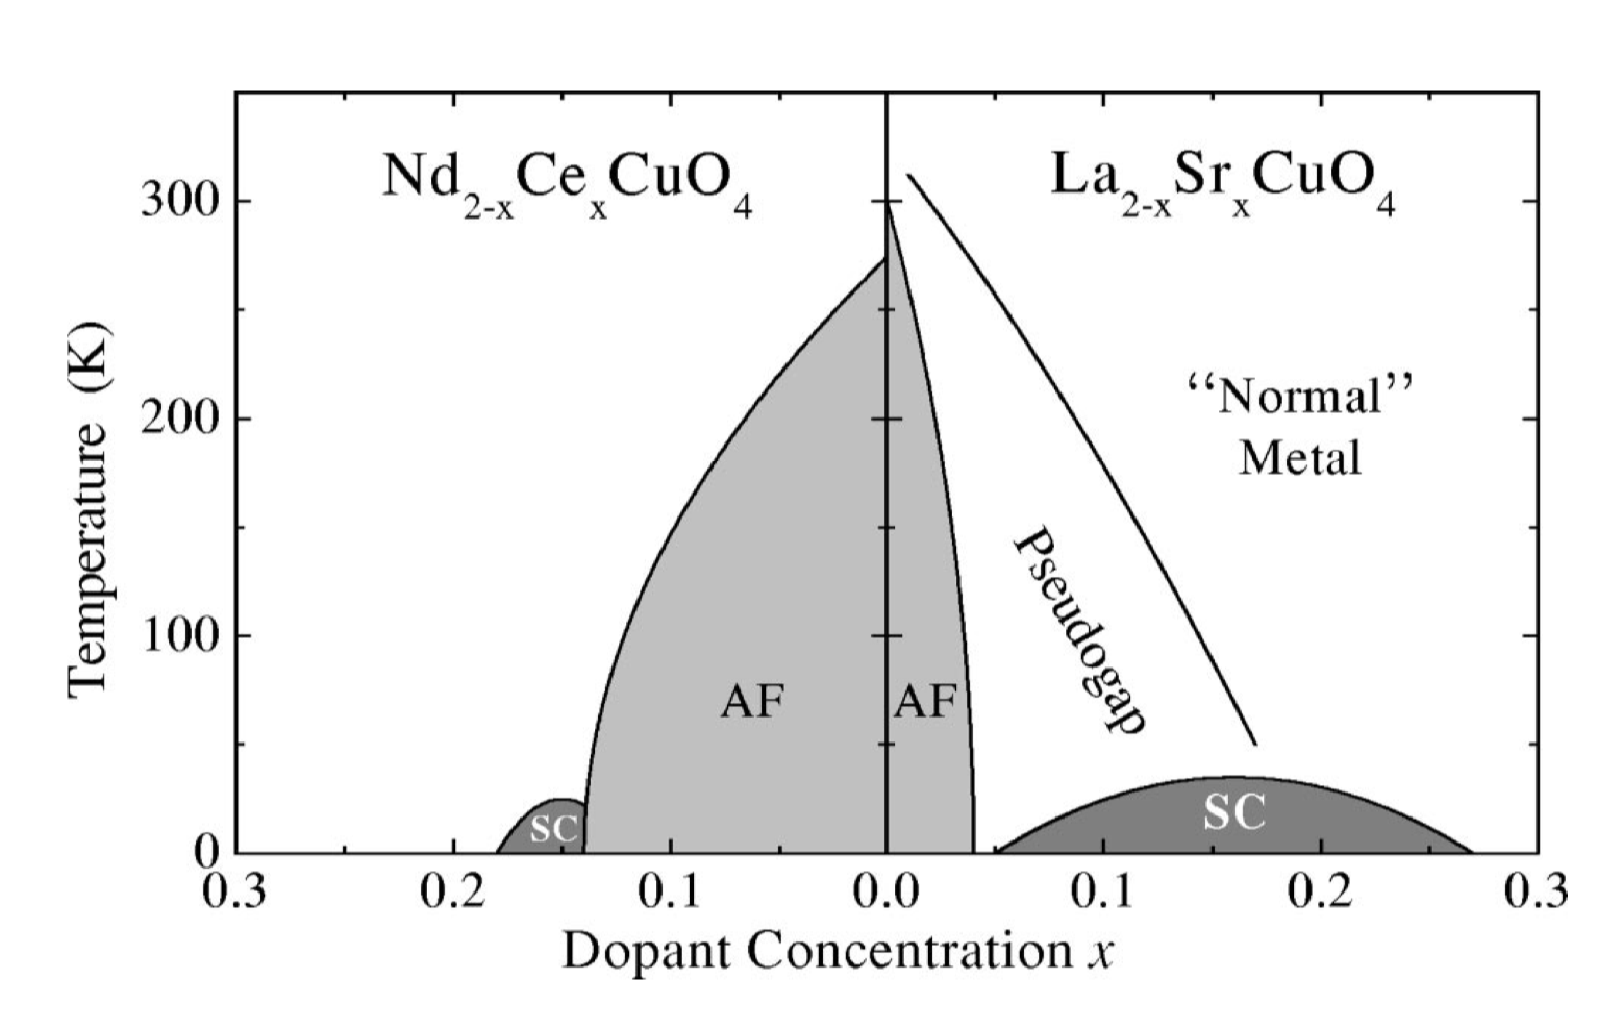
\includegraphics[width=100mm]{Introduction/phase_diagram.eps}
  \end{center}
  \caption{銅酸化物高温超伝導体の典型的な相図\cite{Andrea2003}}
  \label{fig:phase_diagram}
\end{figure}


まず銅酸化物において過渡的な超伝導を実現した報告に関して述べる。Faustiらは常伝導相のある銅酸化物に赤外光パルスを入射することで、過渡的な超伝導相が現れることを示した\cite{Fausti,Hunt2015}。図\ref{fig:phase_diagram2}に彼らが用いた$\rm La_{1.8-x}Eu_{0.2}Sr_{x}CuO_4$の相図を示す\cite{Cavalleri2018}。典型的な銅酸化物超伝導体(図\ref{fig:phase_diagram})と同様にドーム状の構造を持ちつつも、$x=1/8$で転移温度に特異的なへこみが見て取れる。この物質はドープ量$x=1/8$となったとき電荷がストライプ状に配列し、超伝導の発現が阻害されることが知られている(ドープ量1/8問題)。彼らはこのストライプ秩序状態の銅酸化物に対して赤外光パルスを印加し格子振動を励起することで、秩序状態を過渡的に破壊し超伝導を実現した。同様にMitranoらはフラーレンとアルカリ金属のインターカレーション$\rm K_3C_{60}$にも過渡的な超伝導相が現れる可能性を示した\cite{Mitrano2016}。これらはパルスを用いて秩序状態を破壊した結果に生じた超伝導であり、元素置換と異なった、非平衡過程を用いたアプローチである。
\begin{figure}[htb]
    \begin{center}
   \includegraphics[width=70mm]{Introduction/phase_diagram2.eps}
  \end{center}
  \caption{銅酸化物高温超伝導体の典型的な相図\cite{Cavalleri2018}}
  \label{fig:phase_diagram2}
\end{figure}

つぎに非平衡過程を用いて秩序状態を抑制し、準定常的な超伝導状態を実現した報告に関して述べる。
大池らは電荷が配列し電荷秩序状態となった遷移金属ダイカルコゲナイドIrTe$_2$を電流パルスにより加熱・急冷すると、急冷時に電荷秩序状態の発現が阻害され、競合する超伝導状態が現れることを示した\cite{Oike}。この超伝導状態は準安定であり、数週間以上持続する。さらにパルス強度とパルス幅を適切に調整することで、超伝導から電荷秩序状態を復元できることも示した。これらは急加熱・急冷を用いて競合する秩序状態を抑制した結果に生じた超伝導であり、平衡過程からは到達できない状態(超伝導)を実現できる。

以上の非平衡過程を用いた超伝導相へのアプローチは、元素置換と異なり外部制御が可能で、原理的に可逆である。しかしこの可逆的な相制御の成果は、一部の物質によってのみ実現されたものであり、抵抗率変化の比較的小さな金属-超伝導変換を示したものである。したがって応用の範囲に制限があり、現象の原理実証は不完全であるといってよい。
%深ほりする

そこで本研究では非平衡過程を経由することで、よく知られた物質において、超伝導体と半導体を可逆的にスイッチングすることを目指した。半導体は低温で抵抗が大きくなるため、超伝導の間で変換できると大きな抵抗率変化につながる。また誘電体であるため電磁気的な応答も超伝導体と大きく異なる。対象物質としてはスズを選んだ。スズは転移温度286.4Kで、金属と半導体の間の構造変化を伴う一次転移をする。低温で半導体が最安定であるが、金属相も急冷することで準安定となり金属相は臨界温度3.7Kの超伝導体となる。スズは地球上に豊富に存在する元素であり、取り扱いやすく、また人体への毒性もない。筆者らは電流パルスを用いた加熱・急冷により、スズの半導体($\rm \alpha$相)-超伝導体($\rm \beta$相)変換の実証を目的とした。

\subsection{スズの物質特性}
スズは周期表において14族の元素である。図\ref{fig:group14}に14族の物質構造を示した。Geはスズのひとつ上の周期に属し、金属のPbはひとつ下の周期に属する。SiとGe、半導体のスズはダイアモンド構造をとる。金属のスズはPbと同様に金属的な高い導電性を示す。室温付近で金属と半導体のエネルギー差は小さく、どちらも安定に存在する。図\ref{fig:bandgaps}に14族半導体のバンドギャップ$\epsilon_g$と最近接原子間距離$R_{nn}$を示す\cite{Yonezawa}。最近接原子間距離$R_{nn}$が大きいほどバンドギャップは小さくなり、半導体スズはバンドが閉じるギリギリのところにあることが見て取れる。半導体スズのバンドギャップは0.08eVと非常に小さい。温度を上げると半導体スズの$R_{nn}$はさらに大きくなり、バンドが閉じ金属的になる。この半導体-金属転移はブロッホ・ウィルソン転移(タイプ2)と呼ばれる\cite{Yonezawa}。

SiとGeと半導体スズはすべて同一のダイアモンド構造をとることから、半導体スズにSiやGeを少量添加すると安定化する\cite{Ewald1954,Gallerneault1983}。図\ref{fig:Ge_Stabilized_Sn}にGe添加量と半導体-金属転移温度の関係を示した\cite{Vnuk1984}。Ge添加量を1\%程度まで増やすと転移温度が大きくなることが見て取れる。またスズ-Ge共晶点に置けるGe固溶の限界は0.3\%程度と言われている\cite{Thurmond1960}。
%Bulletin of Alloy Phase Diagrams Vol. 5 No. 3 1984

\begin{figure}[htb]]
 \begin{minipage}{0.4\hsize}
  \begin{center}
   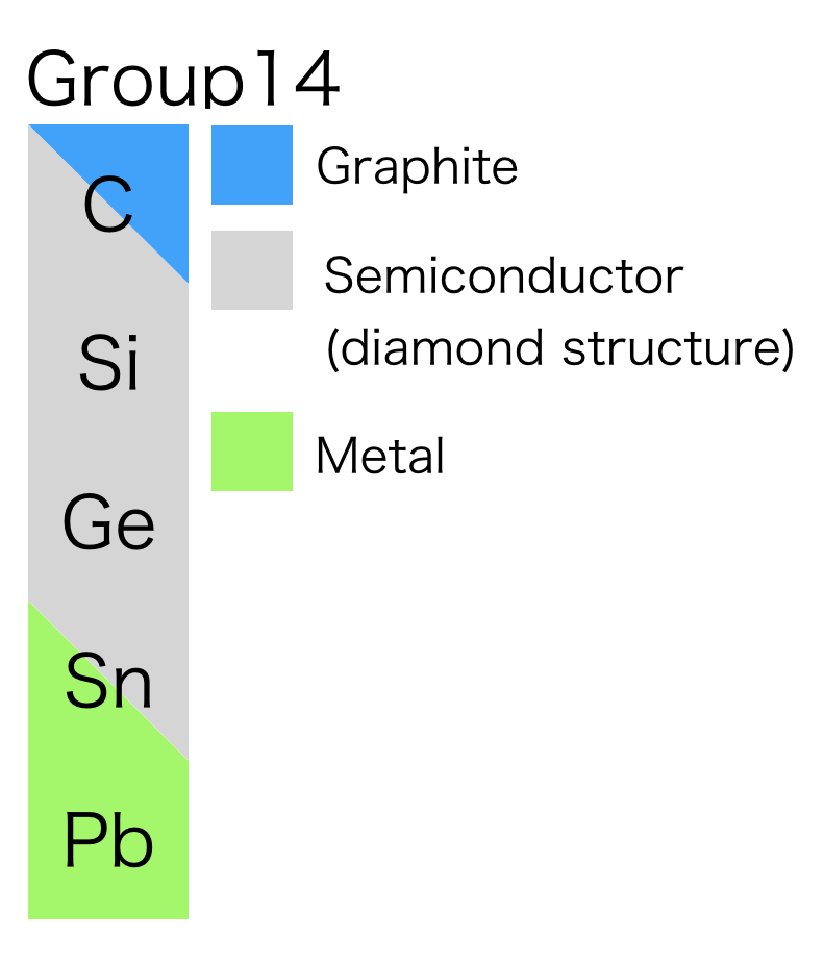
\includegraphics[width=50mm]{experiment/group14.eps}
  \end{center}
  \caption{14族元素の相}
  \label{fig:group14}
 \end{minipage}
 \begin{minipage}{0.6\hsize}
  \begin{center}
   
\includegraphics[width=90mm]{experiment/bandgaps.eps}
  \end{center}
  \caption{14族半導体のバンドギャップ$\epsilon_g$と最近接原子間距離$R_{nn}$\cite{Yonezawa}}
  \label{fig:bandgaps}
 \end{minipage}
\end{figure}

\begin{figure}[htb]
    \begin{center}
   \includegraphics[width=70mm]{experiment/Ge_Stabilized_Sn.eps}
  \end{center}
  \caption{Ge添加量とスズの$\alpha-\beta$転移温度\cite{Vnuk1984}}
  \label{fig:Ge_Stabilized_Sn}
\end{figure}


%スズに関して(構造相転移など)

